\documentclass{standalone}
\usepackage{tikz}
\usetikzlibrary{patterns}
\usetikzlibrary{positioning}
\usetikzlibrary{patterns, positioning}
\usetikzlibrary{shapes.misc}
\usepackage[outline]{contour}
\contourlength{1.5pt} 
\usepackage[sfdefault]{ClearSans}

\begin{document}
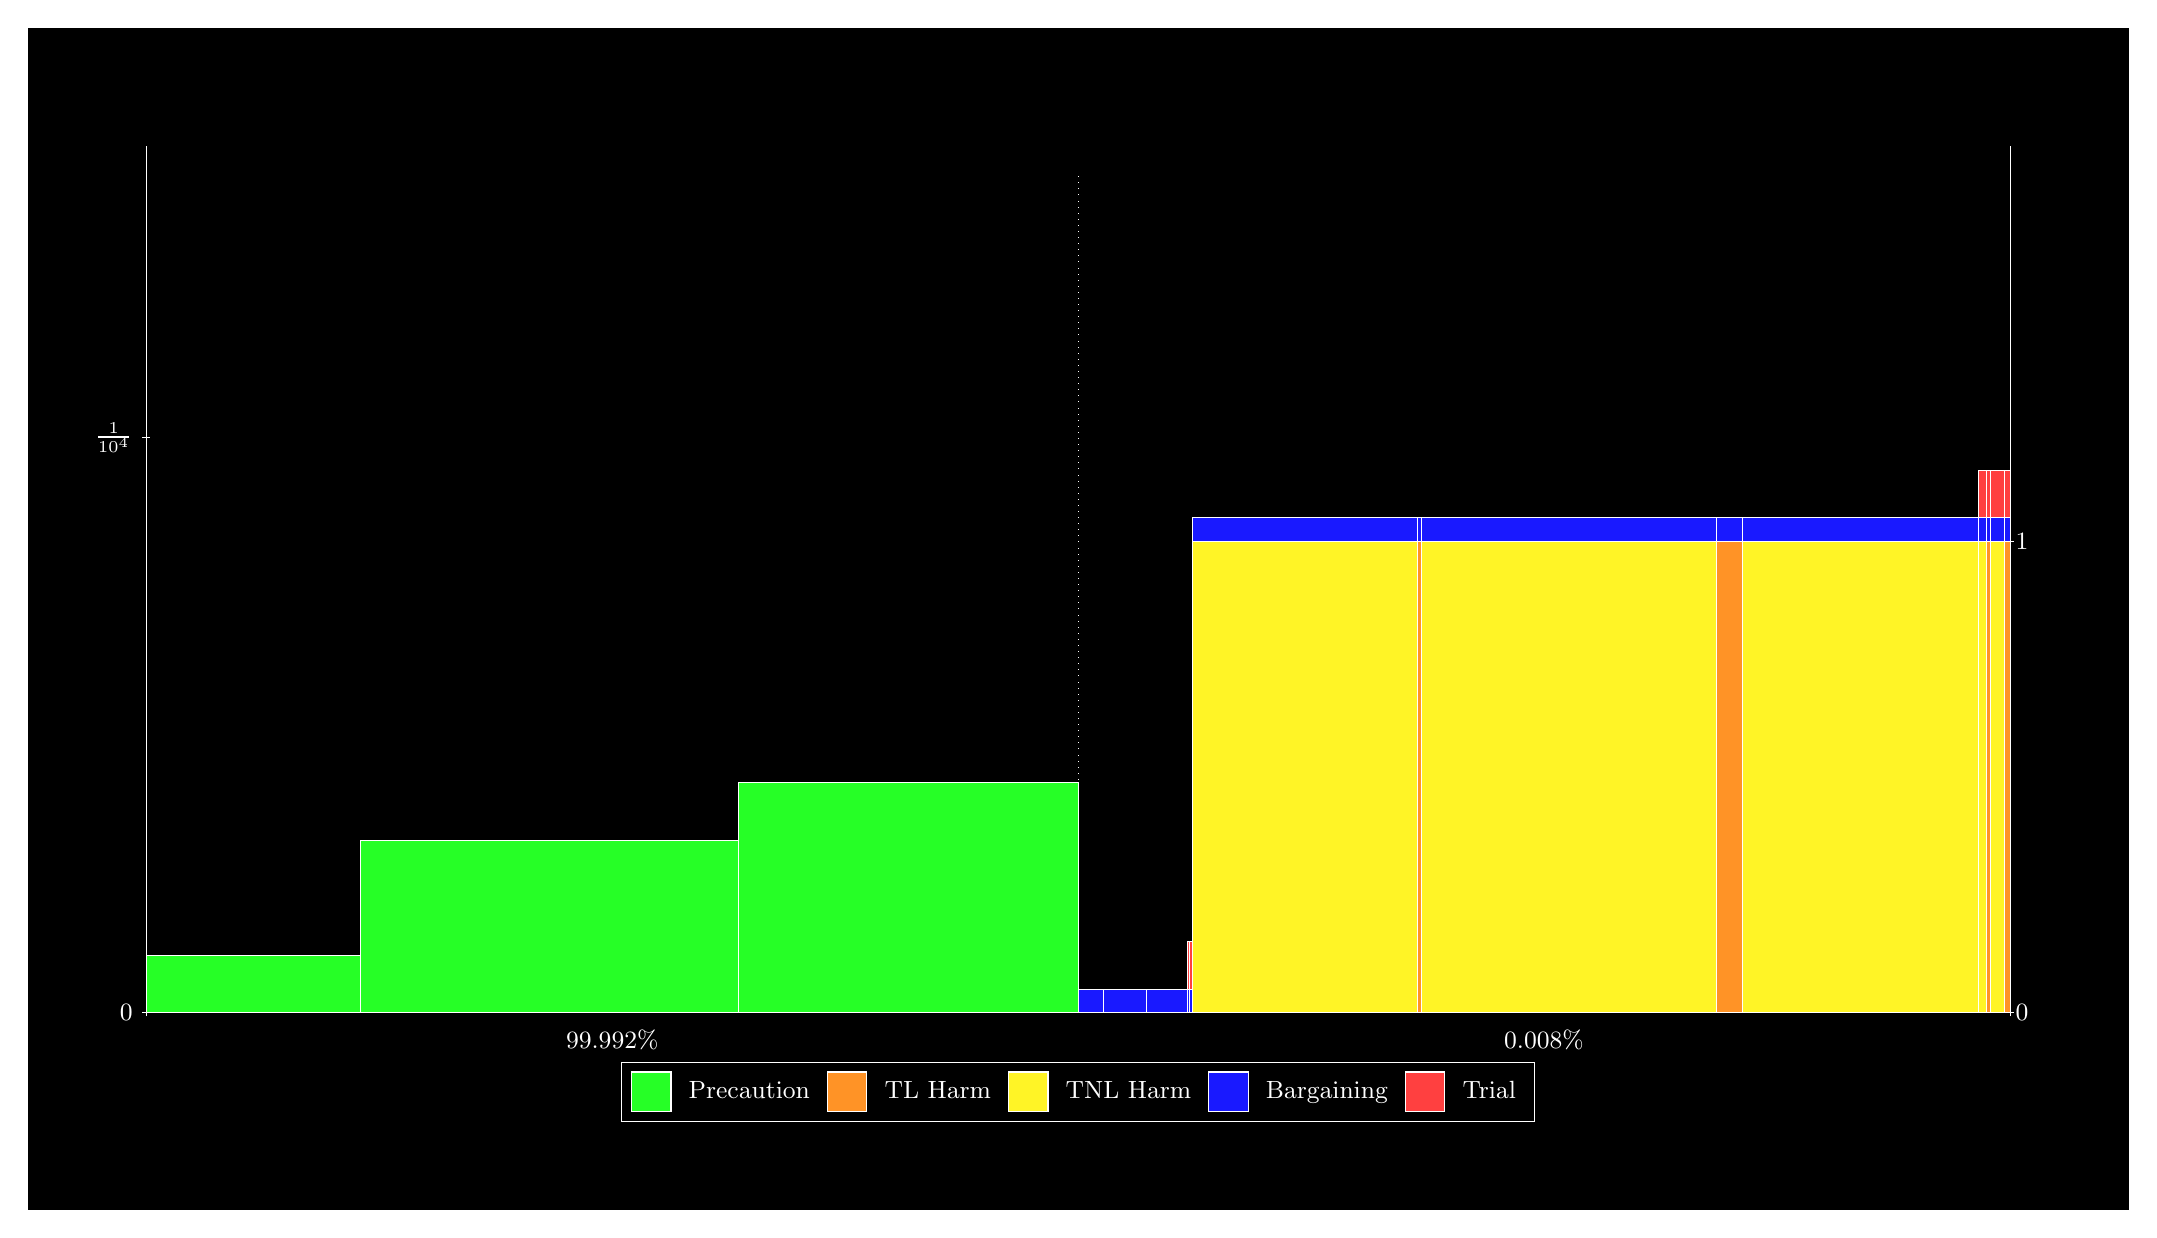
\begin{tikzpicture}
\draw[fill=black] (0,0) rectangle (26.667,15);
\draw[fill=green!85,draw=white,very thin] (1.5,2.5) rectangle (4.2218,3.2304);
\draw[fill=green!85,draw=white,very thin] (4.2218,2.5) rectangle (9.0126,4.6912);
\draw[fill=green!85,draw=white,very thin] (9.0126,2.5) rectangle (13.333,5.4216);
\draw[fill=green!85,draw=white,very thin] (13.333,2.5) rectangle (13.648,2.5001);
\draw[fill=blue!90,draw=white,very thin] (13.333,2.5001) rectangle (13.648,2.7994);
\draw[fill=green!85,draw=white,very thin] (13.648,2.5) rectangle (14.197,2.5002);
\draw[fill=blue!90,draw=white,very thin] (13.648,2.5002) rectangle (14.197,2.7995);
\draw[fill=green!85,draw=white,very thin] (14.197,2.5) rectangle (14.724,2.5002);
\draw[fill=blue!90,draw=white,very thin] (14.197,2.5002) rectangle (14.724,2.7996);
\draw[fill=green!85,draw=white,very thin] (14.724,2.5) rectangle (14.741,2.5001);
\draw[fill=blue!90,draw=white,very thin] (14.724,2.5001) rectangle (14.741,2.7994);
\draw[fill=red!75,draw=white,very thin] (14.724,2.7994) rectangle (14.741,3.3981);
\draw[fill=green!85,draw=white,very thin] (14.741,2.5) rectangle (14.777,2.5002);
\draw[fill=blue!90,draw=white,very thin] (14.741,2.5002) rectangle (14.777,2.7995);
\draw[fill=red!75,draw=white,very thin] (14.741,2.7995) rectangle (14.777,3.3982);
\draw[fill=green!85,draw=white,very thin] (14.777,2.5) rectangle (17.635,2.5001);
\draw[fill=yellow!85,draw=white,very thin] (14.777,2.5001) rectangle (17.635,8.4868);
\draw[fill=blue!90,draw=white,very thin] (14.777,8.4868) rectangle (17.635,8.7861);
\draw[fill=green!85,draw=white,very thin] (17.635,2.5) rectangle (17.694,2.5001);
\draw[fill=orange!85,draw=white,very thin] (17.635,2.5001) rectangle (17.694,8.4868);
\draw[fill=blue!90,draw=white,very thin] (17.635,8.4868) rectangle (17.694,8.7861);
\draw[fill=green!85,draw=white,very thin] (17.694,2.5) rectangle (21.442,2.5002);
\draw[fill=yellow!85,draw=white,very thin] (17.694,2.5002) rectangle (21.442,8.4869);
\draw[fill=blue!90,draw=white,very thin] (17.694,8.4869) rectangle (21.442,8.7863);
\draw[fill=green!85,draw=white,very thin] (21.442,2.5) rectangle (21.762,2.5002);
\draw[fill=orange!85,draw=white,very thin] (21.442,2.5002) rectangle (21.762,8.4869);
\draw[fill=blue!90,draw=white,very thin] (21.442,8.4869) rectangle (21.762,8.7863);
\draw[fill=green!85,draw=white,very thin] (21.762,2.5) rectangle (24.767,2.5002);
\draw[fill=yellow!85,draw=white,very thin] (21.762,2.5002) rectangle (24.767,8.487);
\draw[fill=blue!90,draw=white,very thin] (21.762,8.487) rectangle (24.767,8.7863);
\draw[fill=green!85,draw=white,very thin] (24.767,2.5) rectangle (24.869,2.5001);
\draw[fill=yellow!85,draw=white,very thin] (24.767,2.5001) rectangle (24.869,8.4868);
\draw[fill=blue!90,draw=white,very thin] (24.767,8.4868) rectangle (24.869,8.7861);
\draw[fill=red!75,draw=white,very thin] (24.767,8.7861) rectangle (24.869,9.3848);
\draw[fill=green!85,draw=white,very thin] (24.869,2.5) rectangle (24.922,2.5001);
\draw[fill=orange!85,draw=white,very thin] (24.869,2.5001) rectangle (24.922,8.4868);
\draw[fill=blue!90,draw=white,very thin] (24.869,8.4868) rectangle (24.922,8.7861);
\draw[fill=red!75,draw=white,very thin] (24.869,8.7861) rectangle (24.922,9.3848);
\draw[fill=green!85,draw=white,very thin] (24.922,2.5) rectangle (25.096,2.5002);
\draw[fill=yellow!85,draw=white,very thin] (24.922,2.5002) rectangle (25.096,8.4869);
\draw[fill=blue!90,draw=white,very thin] (24.922,8.4869) rectangle (25.096,8.7863);
\draw[fill=red!75,draw=white,very thin] (24.922,8.7863) rectangle (25.096,9.3849);
\draw[fill=green!85,draw=white,very thin] (25.096,2.5) rectangle (25.167,2.5002);
\draw[fill=orange!85,draw=white,very thin] (25.096,2.5002) rectangle (25.167,8.4869);
\draw[fill=blue!90,draw=white,very thin] (25.096,8.4869) rectangle (25.167,8.7863);
\draw[fill=red!75,draw=white,very thin] (25.096,8.7863) rectangle (25.167,9.3849);
\draw[white,very thin] (1.5,2.5) -- (1.5,13.5);
\draw[white,very thin] (1.45,2.5) -- (1.55,2.5);
\node[font=\small,text=white, anchor=east] at (1.45, 2.5) {0};
\draw[white,very thin] (1.45,9.804) -- (1.55,9.804);
\node[font=\small,text=white, anchor=east] at (1.45, 9.804) {$\frac{1}{10^{4}}$};

\draw[white,dotted,very thin] (13.333,2.83) -- (13.333,13.17);
\draw[white,very thin] (25.167,2.5) -- (25.167,13.5);
\draw[white,very thin] (25.117,2.5) -- (25.217,2.5);
\node[font=\small,text=white, anchor=west] at (25.117, 2.5) {0};
\draw[white,very thin] (25.117,8.4867) -- (25.217,8.4867);
\node[font=\small,text=white, anchor=west] at (25.117, 8.4867) {1};

\draw[white,very thin] (1.5,2.5) -- (25.167,2.5);
\draw[white,very thin] (1.5,2.45) -- (1.5,2.55);
\node[font=\small,text=white, anchor=north] at (1.5, 2.45) {};
\draw[white,very thin] (25.167,2.45) -- (25.167,2.55);
\node[font=\small,text=white, anchor=north] at (25.167, 2.45) {};

\node[font=\small,text=white,anchor=south] at (7.4167, 1.9) {99.992\%};
\node[font=\small,text=white,anchor=south] at (19.25, 1.9) {0.008\%};
\draw (13.3333,2.5) node (B) {};
\begin{scope}[align=center]
\matrix[scale=0.5,draw=white,below=0.5cm of B,nodes={draw},column sep=0.1cm]{
\node[rectangle,draw,minimum width=0.5cm,minimum height=0.5cm,fill=green!85]{}; & \node[draw=none,font=\small,text=white]{Precaution}; &
\node[rectangle,draw,minimum width=0.5cm,minimum height=0.5cm,fill=orange!85]{}; & \node[draw=none,font=\small,text=white]{TL Harm}; &
\node[rectangle,draw,minimum width=0.5cm,minimum height=0.5cm,fill=yellow!85]{}; & \node[draw=none,font=\small,text=white]{TNL Harm}; &
\node[rectangle,draw,minimum width=0.5cm,minimum height=0.5cm,fill=blue!90]{}; & \node[draw=none,font=\small,text=white]{Bargaining}; &
\node[rectangle,draw,minimum width=0.5cm,minimum height=0.5cm,fill=red!75]{}; & \node[draw=none,font=\small,text=white]{Trial}; \\\\
};\end{scope}

\end{tikzpicture}
\end{document}